%%%%%%%%%%%%%%%%
% Latex Header %
%%%%%%%%%%%%%%%%

%%%%%%%%%%%%%%%%%%
% General config %
%%%%%%%%%%%%%%%%%%

\documentclass{article}
\usepackage[margin=1.2in]{geometry}
\usepackage[english]{babel}

%%%%%%%%%%%%
% Packages %
%%%%%%%%%%%%

% Math packages
\usepackage{amsthm}
\usepackage{amsmath,amssymb}
\usepackage{amsfonts,mathtools}
% \usepackage{thmbox}
\usepackage{bm}
\usepackage{proof-at-the-end}

% graphics packages
\usepackage{pict2e,picture}
\usepackage{graphicx}
\usepackage{tikz}
\usetikzlibrary {positioning,graphs,calc,decorations.pathmorphing,shapes,arrows.meta,arrows,shapes.misc}
\usetikzlibrary{topaths,calc}
\usetikzlibrary{fit}
\usepackage{subcaption}
\usepackage{xcolor}
\usepackage{wrapfig}
\usepackage{float}

% custom environments
\usepackage{comment}
\usepackage{enumitem}
\usepackage{epigraph}
\usepackage{environ}
\usepackage{listings}

% Miscellanious packages
\usepackage{lipsum,mwe,abstract}
\usepackage{multicol}
\usepackage{refcount}
\usepackage{hyperref}
\usepackage{censor}
\usepackage[numbers]{natbib}



%%%%%%%%%%%%%%%%%%%
% Custom Commands %
%%%%%%%%%%%%%%%%%%%

% covering relation
\newcommand{\coveringA}{%
  \mathrel{-\mkern-4mu}<%
}
\newcommand{\coveringB}{\mathrel{\text{$\vcenter{\hbox{\pictcoveringB}}$}}}
\newcommand{\pictcoveringB}{%
  \begin{picture}(1em,.5em)
    \roundcap
    \put(0,.25em){\line(1,0){.6em}}
    \put(.6em,.25em){\line(3,1){.4em}}
    \put(.6em,.25em){\line(3,-1){.4em}}
  \end{picture}%
}

% highlight
\newcommand{\highlight}[1]{%
  \par\noindent
  \colorbox{gray!30}{%
    \parbox{\dimexpr\linewidth-2\fboxsep\relax}{%
      #1
    }%
  }}

% custom theorem environments
\theoremstyle{plain}
\newtheorem{theorem}{Theorem}[section]
\newtheorem{corollary}[theorem]{Corollary}
\newtheorem{lemma}[theorem]{Lemma}
\newtheorem{prop}[theorem]{Proposition}

\theoremstyle{definition}
\newtheorem{definition}[theorem]{Definition}
\newtheorem{example}[theorem]{Example}
\newtheorem{property}[theorem]{Property}
\newtheorem{notation}[theorem]{Notation}
\newtheorem{convention}[theorem]{Convention}
\newtheorem{interpretation}[theorem]{Interpretation}
\newtheorem{remark}[theorem]{Remark}
% \newtheorem{question}[theorem]{Question}
\newtheorem{note}[theorem]{Note}

\newtheorem{question}{Question}
\theoremstyle{plain}
\newtheorem{assertion}{Assertion}[question]

\newenvironment{reponse}{\renewcommand{\proofname}{Réponse}\begin{proof}}{\end{proof}}

% special theorems / definitions / lemmas
\newtheoremstyle{specialthm}% name
{\topsep}%   Space above
{\topsep}%   Space below
{\itshape}%  Body font
{}%          Indent amount
{\bfseries}% Theorem head font
{}%          Punctuation after theorem head -- blank
{0.5em}%     Space after theorem head (0.5em is the default)
{{\thmname{#1}\thmnumber{ #2$^{\bm*}\!$}\thmnote{\ \textmd{(#3)}.}}}

\theoremstyle{specialthm}
\newtheorem{sptheorem}[theorem]{Theorem}
\newtheorem{spcorollary}[theorem]{Corollary}
\newtheorem{splemma}[theorem]{Lemma}
\newtheorem{spprop}[theorem]{Proposition}

% special theorems / definitions / lemmas
\newtheoremstyle{specialdef}% name
{\topsep}%   Space above
{\topsep}%   Space below
{}%  Body font
{}%          Indent amount
{\bfseries}% Theorem head font
{}%          Punctuation after theorem head -- blank
{0.5em}%     Space after theorem head (0.5em is the default)
{{\thmname{#1}\thmnumber{ #2$^{\bm*}\!$}\thmnote{\ \textmd{(#3)}.}}}

\theoremstyle{specialdef}
\newtheorem{spdefinition}[theorem]{Definition}
\newtheorem{spproperty}[theorem]{Property}

% abstract customization
\renewenvironment{abstract}
{\small
  \begin{center}
    \bfseries \abstractname\vspace{-.5em}\vspace{0pt}
  \end{center}
  \list{}{
    \setlength{\leftmargin}{20mm}
    \setlength{\rightmargin}{\leftmargin}
  }
\item\relax}
{\endlist}

% special epigraph/acknowledgements
\newenvironment{dedication}
{\clearpage           % we want a new page
  \vspace*{\stretch{1}}% some space at the top
  \itshape             % the text is in italics
  \raggedleft          % flush to the right margin
  \begin{minipage}{0.6\linewidth}
    \parindent=12pt
  }
  {\end{minipage}
  \par % end the paragraph
  \vspace{\stretch{2}} % space at bottom is three times that at the top
  \raggedleft
  \textit{All Finite Lattices are Algebraic Lattices.}\\
  \textit{-- G. Birkhoff}
  \vspace{\stretch{1}}
  \clearpage           % finish off the page
}

% Size for partition
% \def\Bign#1{\mathclose{\hbox{$\left#1\vbox to11.5\p@{}\right.\n@space$}}\mathopen{}}

% equiv class
\def\equivclass{/}


%%%%%%%%%%%%%%
% Title Page %
%%%%%%%%%%%%%%

\title{\Large main}
\date{07/28/21}

\begin{document}

%%%%%%%%%%%%%%
% Title Page %
%%%%%%%%%%%%%%
\begin{titlepage}
  \centering

  % Sorbonne Logo
  
\includegraphics[width=0.4\textwidth]{img/logo_sorbonne.png}

  \vspace{3cm}

  % Title
  {\scshape\LARGE Sorbonne Université \par M1 Androide / IQ\par}
  \vspace{1cm}
  {\scshape\Large MOGPL\par}
  \vspace{3cm}
  {\huge\bfseries Projet - Automne 2021\par}
  \vspace{3cm}
  {\Large \textbf{Hugo \textsc{Abreu}}\par}
  {\Large \textbf{Krisni \textsc{Almehdi}}\par}
  \vspace{2cm}

  % Supervision
  soutenu le 17 Décembre 2021\par
  % \vspace{0.5cm}

  % \textbf{Gonzalo \textsc{de Polavieja}}\par
  % \vspace{1mm}
  % and\par
  % \vspace{1mm}
  % \textbf{Fernando \textsc{Martin-Maroto}}

  \vfill

  % % Champalimaud and Algebraic AI info
  % \begin{minipage}{5cm}
  %   \begin{center}
  %     
\includegraphics[width=0.6\textwidth]{img/champalimaud_logo_square_crop.png}
  %   \end{center}
  %   \textbf{Champalimaud Foundation},\\
  %   Av. Brasília,\\
  %   1400-038 Lisboa
  % \end{minipage}
  % \hfill
  % \begin{minipage}{5cm}
  %   \begin{center}
  %     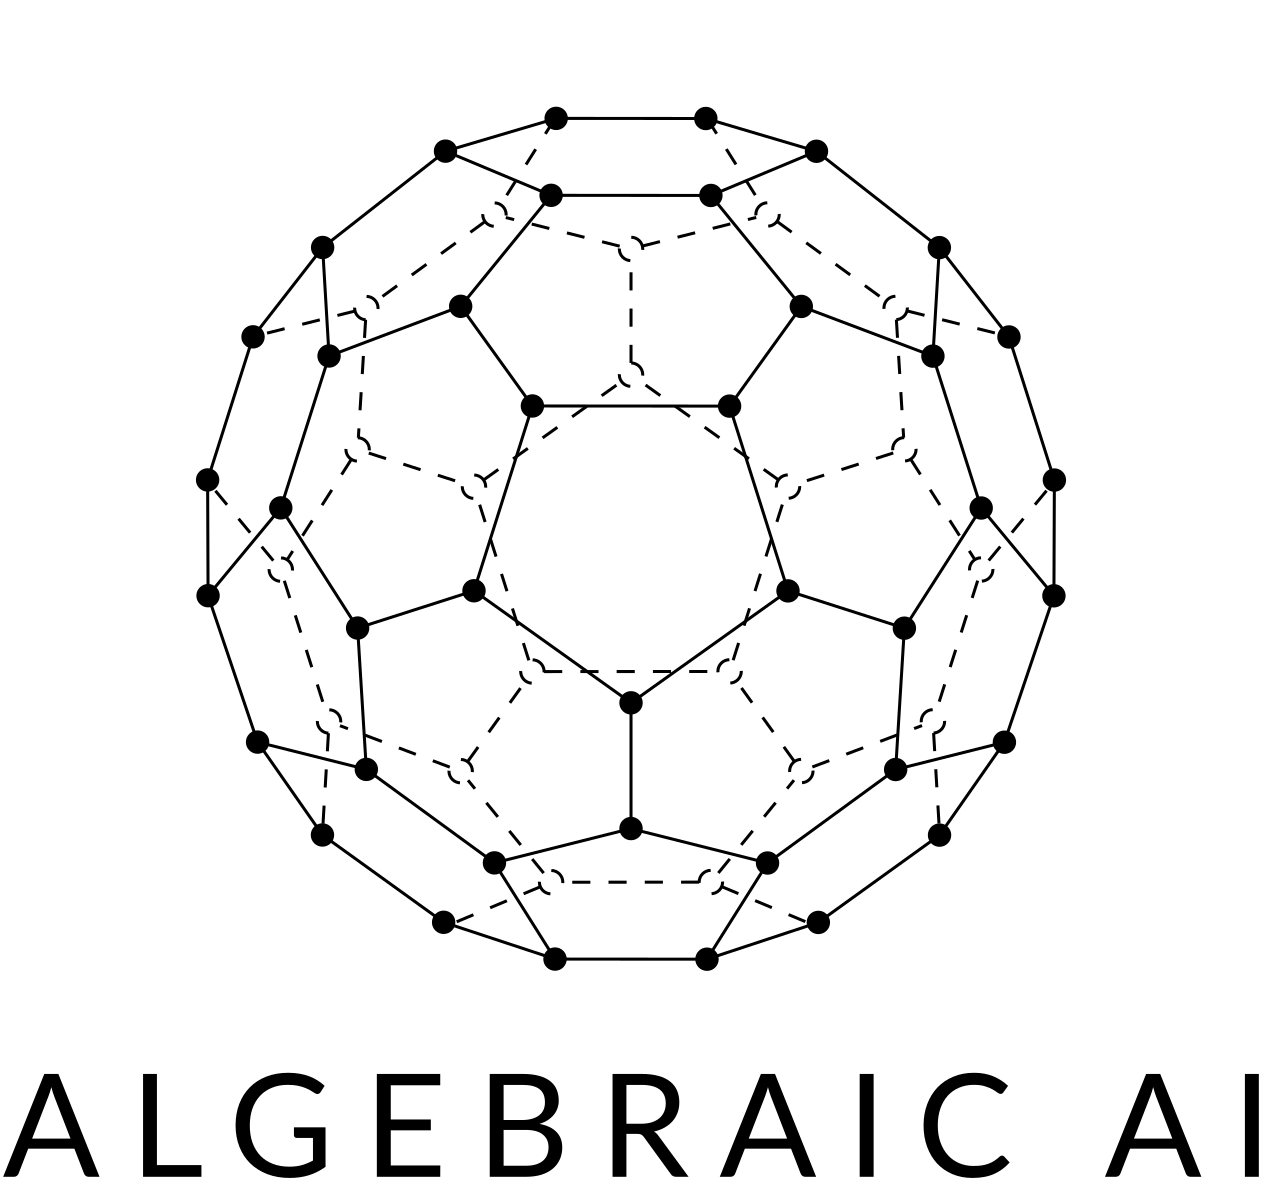
\includegraphics[width=0.6\textwidth]{img/algebraic.png}
  %   \end{center}
  %   \textbf{Algebraic AI},\\
  %   C/ Doctor Fleming 1,\\
  %   28036 Madrid
  % \end{minipage}

\end{titlepage}
\newpage


%%%%%%%%%%%%%%%%%%%%%%%%%%%%
% Acknowledgements / Quote %
%%%%%%%%%%%%%%%%%%%%%%%%%%%%

% \pagenumbering{roman}
% \begin{dedication}
  I want to thank Gonzalo de Polavieja and Fernando Martin Maroto for their
  trust, availability and for providing a very exciting subject for the
  internship. I also want to thank David Mendez for the helpful discussions, and
  Gonçalo Maia Giga, with whom I worked throughout this internship, and who made
  working the entire summer a breeze.

  \vspace{7pt}

  I acknowledge funding from Algebraic AI, provided through the European
  Comission's \textit{H2020 ICT48} project \textit{ALMA: Human Centric Algebraic
    Machine Learning} (grant \#952091).
\end{dedication}



%%%%%%%%%%%%
% Abstract %
%%%%%%%%%%%%

% \begin{abstract}
  % In this report, the theoretical foundations of Algebraic Machine Learning,
  % introduced in \cite{martin-maroto_algebraic_2018} and
  % \cite{martin-maroto_finite_2021}, are studied, and a clear and complete
  % introduction to it is attempted. By
  This report presents a theoretical study of AML (Algebraic Machine Learning), a
  novel approach to Machine Learning introduced by Fernando Martin-Maroto and
  Gonzalo de Polavieja in \cite{martin-maroto_algebraic_2018} et
  \cite{martin-maroto_finite_2021}. Important concepts were singled out,
  implicit prerequisites were explicited, and a more formal connection with
  concepts in Universal Algebra was attempted. An implimentation of full
  crossing, an important operation for AML, was also built.
\end{abstract}

\renewcommand{\abstractname}{Résumé}
\begin{abstract}
  Ce rapport présente une étude théorique d'AML (Machine Learning Algébrique),
  une nouvelle approche au Machine Learning proposée par Fernando Martin-Maroto
  et Gonzalo de Polavieja dans \cite{martin-maroto_algebraic_2018} et
  \cite{martin-maroto_finite_2021}. Les concepts les plus importants ont été mis
  en avant, les prérequis implicites ont été explicités, et plusieurs concepts
  ont été reliés à l'Algèbre Universelle. Une implémentation du ``full
  crossing'', une opération importante pour l'AML, a été réalisée.
\end{abstract}
% \vfill


%%%%%%%%%%%%%%%%%%%%%
% Table of Contents %
%%%%%%%%%%%%%%%%%%%%%

\vspace*{13cm}

\setcounter{tocdepth}{2}
\tableofcontents
\newpage


%%%%%%%%%%%%%%%%%%%%%%%%%%%%%%%%%%%%%%
% ========== Main Content ========== %
%%%%%%%%%%%%%%%%%%%%%%%%%%%%%%%%%%%%%%

\pagenumbering{arabic}
\setcounter{page}{1}
% \vspace*{9.5cm}

% Section 1: Introduction

\section{Introduction}
\label{sec:introduction}

Dans ce projet, on considère des multigraphes orientés pondérés par le temps. Ce
type de graphe est utile notamment pour la plannification temporelle - nous
considèrerons le cas où un réseau de transport aérien est représenté par un tel
graphe.


%%% Local Variables:
%%% mode: latex
%%% TeX-master: "../main"
%%% End:


% Section 2: Préliminaires

\section{Préliminaires}
\label{sec:preliminaires}

\begin{question}
  En utilisant l'instance de la figure de gauche de l'Exemple 1 (dans l'énoncé)
  ou une autre instance, montrer que les assertions suivantes sont vraies.
\end{question}

Par soucis de simplicité et pour être plus concis, une instance alternative est
proposée. Considérons $G_{1}$, le multigraphe orienté pondéré orienté par le
temps donné par le diagramme de la Figure \ref{fig:G1}:

\begin{figure}[h!]
  \centering
  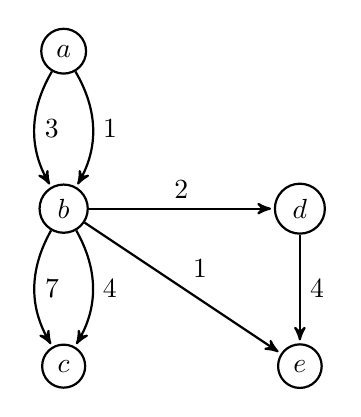
\begin{tikzpicture}[->,>=stealth',shorten >=1pt,auto,node distance=4cm,
    thick,main node/.style={circle,draw,font=\bfseries}]

    \node[main node] (a) at (0,0) {$a$};
    \node[main node] (b) at (0,-2) {$b$};
    \node[main node] (c) at (0,-4) {$c$};
    \node[main node] (d) at (3,-2) {$d$};
    \node[main node] (e) at (3,-4) {$e$};

    \path
    (a) edge [bend left]  node {$1$} (b)
    (a) edge [bend right] node {$3$} (b)
    (b) edge [bend left]  node {$4$} (c)
    (b) edge [bend right] node {$7$} (c)
    (b) edge node {$2$} (d)
    (b) edge node {$1$} (e)
    (d) edge node {$4$} (e);
  \end{tikzpicture}
  \caption{Diagramme représentant le multigraphe pondéré orienté par le temps $G_{1}$}
  \label{fig:G1}
\end{figure}

Le multigraphe $G_1$ sera utilisé pour justifier les assertions suivantes.

\begin{assertion}
  Un sous-chemin préfixe d'un chemin d'arrivée au plus tôt peut ne pas
  être un chemin d'arrivée au plus tôt.
\end{assertion}


\begin{reponse}
  Considérons l'ensemble de chemins $\mathcal{P}(a,c,[0, \infty])$ dans le
  multigraphe $G_{1}$, qui correspond à l'ensemble de tous les chemins
  réalisables de $a$ à $c$ dans $G_{1}$:

  \begin{equation}
    \begin{align}
      \label{eq:1}
      \mathcal{P}(a,c,[0, \infty]) = \{ & P_1 = ((a,b,1,1), (b,c,4,1)), \\
                                        & P_2 = ((a,b,1,1), (b,c,7,1)), \\
                                        & P_3 = ((a,b,3,1), (b,c,4,1)), \\
                                        & P_4 = ((a,b,3,1), (b,c,7,1)) \}.
    \end{align}
  \end{equation}

  Pour déterminer le(s) chemin(s) d'arrivée au plus tôt de $a$ à $c$ dans le
  graphe $G_{1}$, soit un chemin $P$ tel que
  $\mathrm{fin}(P) = \min(\{\mathrm{fin}(P'): P' \in \mathcal{P}(a,c,[0,
  \infty]\})$, calculons les dates de fin pour tout
  $P$ appartenant à $\mathcal{P}(a,c,[0, \infty])$:

  \begin{equation}
    \begin{align}
      \label{eq:2}
      & \mathrm{fin}(P_1) = 4 + 1 = 5, \\
      & \mathrm{fin}(P_2) = 7 + 1 = 8, \\
      & \mathrm{fin}(P_3) = 4 + 1 = 5, \\
      & \mathrm{fin}(P_4) = 7 + 1 = 8.
    \end{align}
  \end{equation}

  Ainsi, $\min(\{5,8,5,8\}) = 5$ et les chemins d'arrivée au plus tôt sont $P_1$
  et $P_3$.

  $P_{3}' = ((a,b,3,1))$, un chemin de $a$ vers $b$, est un sous-chemin préfixe
  (un sous-chemin partant du sommet de départ) de $P_{3}$. Cependant, il existe
  un chemin $P_{a \rightarrow b} = ((a,b,1,1))$ tel que
  \begin{equation}
    \mathrm{fin}(P_{3}') = 3 + 1 = 4 > \mathrm{fin}(P_{a \rightarrow b}) = 1 + 1
    = 2 \text{,}
  \label{eq:4}
  \end{equation}
  donc $P_{3}'$ n'est pas un chemin d'arrivée au plus tôt de $a$ à $b$.

  Ainsi, un sous-chemin préfixe d'un chemin d'arrivée au plus tôt peut ne pas
  être un chemin d'arrivée au plus tôt.
\end{reponse}

\begin{assertion}
  Un sous-chemin postfixe d'un chemin de départ au plus tard peut ne pas être un
  chemin de départ au plus tard.
\end{assertion}

\begin{reponse}
  Considérons de nouveau l'ensemble de chemins $\mathcal{P}(a,c,[0, \infty])$,
  donné en Équation \ref{eq:1}.

  Un chemin de départ au plus tard de $a$ à $c$, dans le multigraphe $G_1$,
  correspond à un chemin $P$ tel que
  $\mathrm{début}(P) = \max(\{\mathrm{début}(P'): P' \in
  \mathcal{P}(a,c,[0, \infty]\})$. On observe facilement que
  \begin{equation}
    \mathrm{début}(P_1) = \mathrm{début}(P_2) = 1 < \mathrm{début}(P_3) =
    \mathrm{début}(P_4) = 3 \text{,}
  \end{equation}
  donc les chemins de départ au plus tard entre $a$ et $c$ sont $P_3$ et $P_4$.

  $P_{3}'' = ((b,c,4,1))$, un chemin de $b$ vers $c$, est un sous-chemin
  postfixe (un sous-chemin partant du sommet final) de $P_3$. Cependant, il
  existe un chemin $P_{b \rightarrow c} = ((b,c,7,1))$ tel que
  \begin{equation}
    \mathrm{début}(P_{3}'') = 3 < \mathrm{début}(P_{b \rightarrow c}) = 7
    \label{eq:5}
  \end{equation}
  donc $P_{3}''$ n'est pas un chemin de départ au plus tard de $b$ à $c$.

  Ainsi, un sous-chemin postfixe d'un chemin de départ au plus tard peut ne pas
  être un chemin de départ au plus tard.
\end{reponse}

\begin{assertion}
  Un sous-chemin d'un chemin le plus rapide peut ne pas être un chemin le plus
  rapide.
  \label{assert:rapide}
\end{assertion}

\begin{reponse}
  Considérons les chemins de $a$ à $d$ dans $G_{1}$:
  \begin{equation}
    \mathcal{P}(a,d,[0, \infty]) = \{P_5 = ((a,b,1,1),(b,d,2,1),(d,e,4,1))\} \text{.}
    \label{eq:6}
  \end{equation}

  Comme il n'existe qu'un seul chemin réalisable, c'est forcément un chemin le
  plus rapide de $a$ à $d$, un chemin $P$ tel que
  $\mathrm{durée}(P) = \min(\{\mathrm{durée}(P'): P' \in \mathcal{P}(a,d,[0,
  \infty]) \})$.

  $P_{5}' = ((b,d,2,1),(d,e,4,1))$, un chemin de $b$ à $e$, est un sous-chemin
  de $P_5$. Cependant, il existe un chemin $P_{b \rightarrow e} = ((b,e,1,1))$
  de $b$ vers $e$ tel que
  \begin{equation}
    \mathrm{durée}(P_{5}') = (4+1) - 1 = 4 > \mathrm{durée}(P_{b \rightarrow e}) = (1+1) - 1 = 1 \text{,}
    \label{eq:3}
  \end{equation}
  donc $P_{5}'$ n'est pas un chemin le plus rapide de $b$ à $e$.

  Ainsi, un sous-chemin d'un chemin le plus rapide peut ne pas être un chemin le
  plus rapide.
\end{reponse}

\begin{assertion}
  Un sous-chemin d'un plus court chemin peut ne pas être un plus court chemin.
\end{assertion}

\begin{reponse}
  Considérons de nouveau les chemins $\mathcal{P}(a,d,[0, \infty])$ de $a$ vers
  $d$ donnés en Équation \ref{eq:6}.

  De même, comme il n'existe qu'un seul chemin réalisable, $P_5$ est forcément
  le chemin le plus court: un chemin $P$ tel que
  $\mathrm{dist}(P) = \min(\{\mathrm{dist}(P'): P' \in \mathcal{P}(a,d,[0,
  \infty]) \})$.

  Considérons de nouveau les chemins $P_{5}''$ et $P_{b \rightarrow e}$ donnés
  en Assertion \ref{assert:rapide}.
  \begin{equation}
    \mathrm{dist}(P_{5}') = 1 + 1 = 2 > \mathrm{dist}(P_{b \rightarrow e}) = 1 \text{,}
    \label{eq:3}
  \end{equation}
  donc $P_{5}'$ n'est pas un chemin le plus court de $b$ à $e$.

  Ainsi, un sous-chemin d'un chemin le plus court peut ne pas être un chemin le
  plus court.

\end{reponse}

%%% Local Variables:
%%% mode: latex
%%% TeX-master: "../main"
%%% End:


% Section 3: Algorithmes de plus court chemin dans des multigraphes orientés
% pondérés par le temps

\section{Algorithmes de plus court chemin dans des multigraphes orientés pondérés par le temps}
\label{sec:algos}


%%% Local Variables:
%%% mode: latex
%%% TeX-master: "../main"
%%% End:



% Section 4: Conclusion

\section{Conclusion}
\label{sec:conclusion}


%%% Local Variables:
%%% mode: latex
%%% TeX-master: "../main"
%%% End:


%%%%%%%%%%%%%%
% References %
%%%%%%%%%%%%%%

% \addcontentsline{toc}{section}{References}
% \bibliographystyle{acm}
% \bibliography{misc/citations}
% \newpage


%%%%%%%%%%%
% Annexes %
%%%%%%%%%%%

% \appendix
% \setcounter{page}{1}
% \pagenumbering{roman}

% \addtocontents{toc}{\protect\setcounter{tocdepth}{1}}

% \section{Proofs}
% \printProofs
% \input{sections/appendix}

\end{document}

%%% Local Variables:
%%% mode: latex
%%% TeX-master: t
%%% End:
